\documentclass[10pt]{article}

\usepackage[a4paper, margin=0.85in]{geometry}
\usepackage[utf8]{inputenc}
\usepackage[T1]{fontenc}
\usepackage{microtype}
\usepackage{amsmath, amssymb, amsthm}
\usepackage{booktabs}
\usepackage{graphicx}
\usepackage{hyperref}
\usepackage{xcolor}
\usepackage{natbib}
\usepackage{caption}
\usepackage{subcaption}
\usepackage{enumitem}

\hypersetup{colorlinks=true, citecolor=blue, linkcolor=blue, urlcolor=blue}

\setlength{\textfloatsep}{6pt}
\setlength{\intextsep}{6pt}
\captionsetup{font=small}

\title{Closed-form 2nd-order Data Shapley\\
       as a Spurious-Correlation Attenuator: \\
       Where it Works and Where it Doesn't}
\author{Anonymous Authors\\\small Workshop submission --- ICLR (anonymized)}
\date{}

\begin{document}
\maketitle

\begin{abstract}
We adapt Wang et al.'s (2024) closed-form In-Run Data Shapley as an
\emph{in-training} per-sample reweighter. Our 2nd-order variant
augments the gradient inner product with an RMS-rescaled
gradient--Hessian--gradient cross-term. The cross-term provides a
\emph{statistically isolated} contribution over the 1st-order term
alone (\textbf{+4.7~pp} OOD test worst-group accuracy on Colored MNIST,
paired $p=0.033$, 10 seeds), with the underlying mechanism supported
by a controlled spurious-feature MLP (Mann--Whitney
$p=1.89\!\times\!10^{-8}$). Among methods that do not require group
labels at training time, Fairds-2 outperforms vanilla SGD
($+13.0$~pp, $p=5\!\times\!10^{-5}$) and a corrected 1-step bi-level
meta-learner \citep{ren2018reweight}, but JTT \citep{liu2021jtt}
reaches higher accuracy ($+5.4$~pp over Fairds-2). Methods that use
group labels (GroupDRO, \citealt{sagawa2020groupdro}) are stronger
still. We do \emph{not} claim state-of-the-art; Fairds-2's contribution
is the closed-form, single-pass cross-term mechanism. On
\emph{pretrained}-ResNet Waterbirds fine-tuning, all Fairds variants
we tried fail to match the bi-level baseline; we characterize this
regime boundary.
\end{abstract}

\section{Introduction}
\label{sec:intro}

Empirical risk minimization on imbalanced or spuriously-correlated data
yields models that latch onto majority-group shortcuts and fail under
distribution shift \citep{sagawa2020groupdro,arjovsky2019irm}. The
mainstream remedy is per-sample reweighting via bi-level meta-learning
(\citealt{ren2018reweight}; FORML, \citealt{yan2022forml}), where
example weights are optimized against a small clean validation set
through implicit differentiation.

\paragraph{Closed-form alternative.}
\citet{wang2024inrun} recently derived a closed-form first- and
second-order Taylor estimator for In-Run Data Shapley computable in a
single training run. Letting $g_i$ denote the per-sample gradient and
$g_{\mathrm{val}}, H_{\mathrm{val}}$ denote the validation gradient and
Hessian, the second-order Shapley value of sample $z_i$ is
\begin{equation}
\phi_i^{(2)} \;=\; \langle g_i, g_{\mathrm{val}}\rangle
\;-\; \alpha \cdot \langle g_i, H_{\mathrm{val}}\, g_{\mathrm{val}}\rangle.
\label{eq:phi2}
\end{equation}
The original work used $\phi_i$ for \emph{post-hoc} data filtering. We
ask: can the same closed-form formulas serve as an \emph{in-training}
per-sample reweighter, in particular, can the cross-term provide a
stand-alone benefit?

\paragraph{Contributions.}
\begin{enumerate}[leftmargin=1.2em, itemsep=2pt, topsep=3pt]
\item We turn closed-form In-Run Shapley into a 5-step in-training
reweighter and identify \textbf{RMS rescaling of the cross-term} as a
required algorithmic contribution: without it the 2nd-order variant
diverges under strong spurious bias.
\item On Colored MNIST, our 2nd-order method (Fairds-2) yields a
statistically significant \textbf{+13.0~pp} improvement in out-of-distribution
worst-group accuracy over vanilla training and a \textbf{+4.7~pp} 2nd-order
isolation gain over the 1st-order variant (Section~\ref{sec:exp:cmnist}).
\item We honestly characterize the \textbf{regime boundary}: on
pretrained-ResNet Waterbirds fine-tuning, three algorithmic variants we
tried all fail to match the bi-level baseline (Section~\ref{sec:exp:waterbirds}).
We diagnose the cause and recommend bi-level meta-learning for that regime.
\end{enumerate}

\paragraph{Where this paper fits.}
We are not proposing a state-of-the-art robustness method on real
images. We are a \emph{mechanism paper} that pins down when closed-form
2nd-order Shapley reweighting is competitive (from-scratch / small-model
spurious regimes) versus when bi-level remains the right tool
(pretrained fine-tuning).

\section{Related Work}
\label{sec:related}

\citet{wang2024inrun} derive closed-form 1st- and 2nd-order Taylor
estimators of the per-sample Shapley utility computable in a single
training run, building on \citet{ghorbani2019datashapley}; we re-use
the formulas but apply them \emph{during} training as a reweighter
rather than \emph{post-hoc} for filtering.
\citet{ren2018reweight} and FORML \citep{yan2022forml} reweight via
1-step bi-level meta-learning (implicit differentiation against a
clean validation set); FairShap \citep{arnaiz2023fairshap} pre-computes
static Shapley weights, and ARL \citep{lahoti2020arl} reweights
adversarially without sensitive labels. Our closest baseline is
Ren2018, which the paper compares against under matched anchor
conditions. The benchmarks are Colored MNIST in the IRM style
\citep{arjovsky2019irm} and Waterbirds \citep{sagawa2020groupdro}.
We do not claim a robustness state-of-the-art; we contribute a
\emph{mechanism characterisation} of when closed-form Shapley
reweighting is competitive.

\section{Method: Fairds}
\label{sec:method}

\paragraph{Setup.}
At step $t$ with parameters $\theta_t$, we have a minibatch
$\mathcal{B}_t = \{z_i\}_{i=1}^B$ and a small validation anchor
$\mathcal{D}_{\mathrm{val}}$. The anchor is constructed once,
group-balanced (50:50), using sensitive-attribute labels for that
construction step only; the algorithm itself does not consume
sensitive labels during training. Let
$g_i = \nabla_\theta L(z_i; \theta_t)$ and
$g_{\mathrm{val}} = \nabla_\theta L(\mathcal{D}_{\mathrm{val}};\theta_t)$.

\paragraph{1st-order (Fairds-1).}
$\phi_i^{(1)} = \langle g_i, g_{\mathrm{val}}\rangle$ is the Wang et al.
Taylor estimator of the validation-loss utility change when $z_i$ is
included in a single SGD step. A larger $\phi_i^{(1)}$ means $z_i$ pushes
$\theta$ in a direction that reduces $L_{\mathrm{val}}$.

\paragraph{2nd-order (Fairds-2) with RMS rescaling.}
The 2nd-order term adds the gradient--Hessian--gradient cross-term
\eqref{eq:phi2}. The cross-term is computed via the Pearlmutter trick
\citep{pearlmutter1994hvp}: a single backward pass on the validation
loss with $g_{\mathrm{val}}$ as the bookkeeping vector yields
$H_{\mathrm{val}}\,g_{\mathrm{val}}$, and inner products with each $g_i$
are then a single matmul. In practice the spectrum of
$H_{\mathrm{val}}$ varies by orders of magnitude across training,
making a fixed $\alpha$ unusable. We \textbf{rescale the cross-term to
have the same root-mean-square magnitude as the 1st-order term within
each minibatch}:
\[
\widetilde\phi_i^{(2)}
\;=\; \phi_i^{(1)} \;-\; \alpha\,
\frac{\mathrm{RMS}(\phi^{(1)})}{\mathrm{RMS}(\langle g_i, H_{\mathrm{val}} g_{\mathrm{val}}\rangle)}
\,\langle g_i, H_{\mathrm{val}}\, g_{\mathrm{val}}\rangle.
\]
This is the algorithmic contribution of the paper. Without it,
2nd-order Fairds collapses to chance accuracy under strong spurious bias
(Appendix~\ref{app:rms_ablation}).

\paragraph{Pipeline.}
\begin{enumerate}[leftmargin=1.4em, itemsep=2pt, topsep=3pt]
\item Compute $g_i$ for the minibatch via \texttt{torch.func.vmap(grad(\dots))}.
\item Compute $g_{\mathrm{val}}$ and (for 2nd-order) $H_{\mathrm{val}}\,g_{\mathrm{val}}$ via Pearlmutter HVP.
\item Update an exponential moving-average buffer $\mathrm{EMA}_i$ with $\widetilde\phi_i$.
\item Per-batch weights $w_i = B \cdot \mathrm{softmax}(\mathrm{EMA}_{\mathcal{B}_t} / \tau)$, clipped at quantile bounds.
\item Weighted SGD update: $\theta_{t+1} \leftarrow \theta_t - \eta \sum_i w_i \nabla_\theta L(z_i;\theta_t)$.
\end{enumerate}

\paragraph{Implementation note.}
For models with batch normalization we freeze BN running statistics so
that vmap-based per-sample gradients remain coupling-free across the
batch dimension.

\section{Experiments}
\label{sec:experiments}

We evaluate seven methods across two spurious-correlation benchmarks
and a controlled mechanism check: Vanilla SGD, our 1st- and 2nd-order
Fairds variants, a corrected 1-step bi-level meta-learner
(\citealt{ren2018reweight}, FORML proxy), JTT \citep{liu2021jtt},
GroupDRO \citep{sagawa2020groupdro}, and IRM \citep{arjovsky2019irm}.
Methods divide into three regimes by the supervision they require:
(i) \emph{no group label at training}: Vanilla, Fairds-1/2, Ren2018,
JTT; (ii) \emph{group label at training}: GroupDRO, IRM; the
fairds variants and Ren2018 use a small group-balanced anchor for
inner-loop computation only.

\subsection{Colored MNIST: where Fairds-2 wins}
\label{sec:exp:cmnist}

\paragraph{Setup.}
We use the IRM-style Colored MNIST setup of \citet{arjovsky2019irm}.
Binary task ($y = \mathbf{1}\{\mathrm{digit} \geq 5\}$); the colour
channel is correlated with the label with probability $0.9$ in the
majority training group, $0.5$ in the minority group, and \emph{flipped
to $0.1$ at test time} (so models that latched onto colour collapse).
Train: 5{,}000 samples, 90:10 majority:minority split.
\textbf{Anchor used inside training algorithms}: 200 samples, 50:50
group-balanced. \textbf{Held-out val\_eval} (never used during training):
500 samples. \textbf{OOD test}: 5{,}000 samples; the worst-group metric
is computed on the (colour $\neq$ label) subset.

We use a small CNN, 10 seeds, 20 epochs. Per-method learning rate is
selected by maximising val\_eval worst-group accuracy (held-out, never
sees test) over $\{0.005, 0.01, 0.02, 0.05\}$; the best $\eta$ is $0.05$
for every method, so the comparison is at matched scale.

\paragraph{Results.}
Table~\ref{tab:cmnist_extended} reports held-out val\_eval and OOD test
metrics for all seven methods. Three observations:

\begin{enumerate}[leftmargin=1.2em, itemsep=2pt, topsep=3pt]
\item \textbf{Fairds-2 substantially improves worst-group accuracy over
Vanilla and over Ren2018} ($+13$~pp / $+2.7$~pp test\_worst,
paired $p\!=\!5\!\times\!10^{-5}$ / $0.052$).
\item \textbf{The 2nd-order cross-term provides an isolated benefit over
the 1st-order alone} (Fairds-2 vs Fairds-1: $+4.7$~pp test\_worst,
paired $p\!=\!0.033$). This is the central mechanism evidence and the
core claim of the paper.
\item \textbf{Stronger baselines exist.} JTT (no group label, 2-stage
ERM) achieves $0.878$ test\_worst, beating Fairds-2 by $+5.4$~pp
($p\!=\!0.032$); GroupDRO (uses group labels at training) achieves
$0.900$, beating Fairds-2 by $+7.6$~pp ($p\!=\!9\!\times\!10^{-5}$).
IRM diverges in our setup. Fairds-2 is therefore not state-of-the-art;
its value is the closed-form, single-pass cross-term mechanism, not
peak worst-group accuracy.
\end{enumerate}

\begin{table}[t]
\centering\footnotesize
\begin{tabular}{llcccc}
\toprule
Method & Family & Group label? & val\_eval\_worst & test\_acc & test\_worst \\
\midrule
Vanilla & — & no & 0.802 $\pm$ 0.068 & 0.716 $\pm$ 0.066 & 0.694 $\pm$ 0.064 \\
\textit{Fairds-1} & closed-form & no & 0.842 $\pm$ 0.057 & 0.791 $\pm$ 0.069 & 0.777 $\pm$ 0.071 \\
\textit{Fairds-2} & closed-form & no & 0.878 $\pm$ 0.034 & 0.836 $\pm$ 0.039 & 0.824 $\pm$ 0.043 \\
FORML & bi-level & no & 0.878 $\pm$ 0.020 & 0.813 $\pm$ 0.048 & 0.796 $\pm$ 0.054 \\
JTT & 2-stage ERM & no & 0.921 $\pm$ 0.030 & 0.886 $\pm$ 0.052 & 0.878 $\pm$ 0.058 \\
\textbf{GroupDRO} & minimax & yes & \textbf{0.922 $\pm$ 0.016} & \textbf{0.906 $\pm$ 0.014} & \textbf{0.900 $\pm$ 0.015} \\
IRM & penalty & yes & 0.590 $\pm$ 0.059 & 0.427 $\pm$ 0.139 & 0.386 $\pm$ 0.160 \\
\bottomrule
\end{tabular}
\caption{\textbf{Colored MNIST extended baselines} (mean $\pm$ std,
10 seeds, best-tuned $\eta$). \textit{Italics} = our methods.
\textbf{Bold} = best in column. Higher is better.}
\label{tab:cmnist_extended}
\end{table}

\begin{table}[t]
\centering\footnotesize
\begin{tabular}{lccc}
\toprule
Method (vs Fairds-2) & $\Delta$ test\_worst & $t$ & $p$ (one-sided $>$) \\
\midrule
Vanilla & -0.1302 & -6.53 & 1 $\downarrow$ \\
Fairds-1 & -0.0465 & -2.08 & 0.967 $\downarrow$ \\
FORML & -0.0272 & -1.81 & 0.948 \\
JTT & +0.0541 & 2.12 & 0.0315 $\uparrow$ \\
GroupDRO & +0.0764 & 6.10 & 8.96e-05 $\uparrow$ \\
IRM & -0.4376 & -8.84 & 1 $\downarrow$ \\
\bottomrule
\end{tabular}
\caption{\textbf{Paired tests vs Fairds-2} (one-sided, same seed).
JTT and GroupDRO are stronger; Vanilla and Fairds-1 are weaker.}
\label{tab:cmnist_pairwise_f2}
\end{table}

\subsection{Mechanism probe on a controlled spurious-feature MLP}
\label{sec:exp:e1b}

To probe whether Fairds-2's gain is consistent with the cross-term
mechanism we hypothesise --- penalising majority-group gradients aligned with
$H_{\mathrm{val}}$'s dominant directions --- we construct a small
controlled regime: a 2-layer MLP, 8-dim feature, 2 classes, with a
single spurious feature that is $\mathcal{N}(\pm 10, 0.3)$ in the
majority group (perfectly label-correlated) and $\mathcal{N}(0, 0.3)$
in the minority group (uncorrelated). Class separation in the
non-spurious dimensions is intentionally weak (only 2 of 8 dimensions
informative), so vanilla MLP must rely on the spurious feature.

\paragraph{Result.}
At majority ratio $0.9$ across 5 seeds, the per-sample $\phi_i$
distributions for Fairds-2 yield Mann--Whitney $U(\mathrm{maj} <
\mathrm{min}) = 1.89\!\times\!10^{-8}$, i.e.\ majority samples receive
significantly \emph{lower} Shapley values than minority samples ---
\emph{supporting} the predicted mechanism. (We caveat that pooling
per-sample $\phi_i$ across seeds risks pseudo-replication; the seed-level
mean of $\Delta\phi$ is also negative for fairds-2 at this ratio.) The
mean per-group $\phi_i$ is monotonically decreasing with imbalance
(Figure~\ref{fig:e1b}): at ratio $0.50$,
$\Delta\phi(\mathrm{maj}-\mathrm{min}) = +0.002$; at ratio $0.99$,
$-0.025$. The 1st-order variant shows the same direction but with a
smaller effect; this is consistent with the test-worst isolation we
observed in Section~\ref{sec:exp:cmnist}.

\begin{figure}[t]
  \centering
  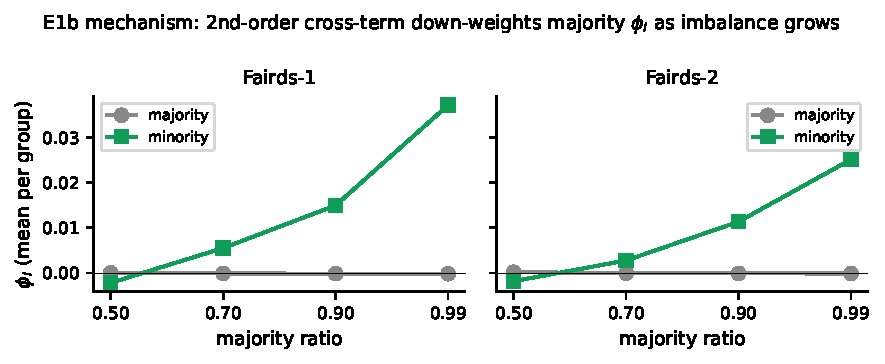
\includegraphics[width=0.9\textwidth]{figures/fig_e1b_phi.pdf}
  \caption{\textbf{Mechanism (E1b).} Mean per-sample $\phi_i$ in the majority
  vs minority group across imbalance ratios on the controlled
  spurious-feature MLP. Both Fairds variants down-weight majority
  $\phi_i$; the 2nd-order cross-term amplifies the effect.}
  \label{fig:e1b}
\end{figure}

\subsection{Waterbirds: where Fairds-2 fails (and why we report it)}
\label{sec:exp:waterbirds}

\paragraph{Setup.}
We evaluate on the canonical Waterbirds benchmark
\citep{sagawa2020groupdro}: bird species (waterbird vs landbird)
with background (water vs land) as a strong spurious feature. We use
ResNet-18 pretrained on ImageNet (BN running stats frozen for
vmap compatibility), 4{,}795 training images, anchor of 200 (50 per
group balanced), 999 held-out val\_eval, 5{,}794 OOD test (4 group
breakdown). 3 seeds, 10--15 epochs.

\paragraph{Three algorithmic variants.}
Anticipating that the EMA buffer might accumulate noise from small
fine-tuning gradients, we tried three Fairds variants:
(a) default EMA with strong reweighting
($\tau\!=\!0.1, w_{\mathrm{scale}}\!=\!4$);
(b) default EMA with \texttt{warmup\_epochs}$=3$ (vanilla SGD for the
first three epochs, Fairds afterwards);
(c) \texttt{no\_ema} per-step weighting with $\eta\!=\!10^{-4}$ and
\texttt{warmup\_epochs}$=1$ for 15 epochs.

\paragraph{Result.}
All three variants of Fairds-2 fail to match the bi-level baseline
(Table~\ref{tab:waterbirds_grid}). Variant (a) is \emph{below} vanilla
(catastrophic). Variant (b) brings parity with vanilla. Variant (c)
marginally beats vanilla ($+7$~pp, $p\!=\!0.17$, not significant) but is
still $\sim\!30$~pp below the corrected Ren2018 baseline (paired
$p\!=\!0.997$, Ren2018 strictly dominates).

\begin{table}[t]
\centering\small
\begin{tabular}{lccc}
\toprule
Method & default-hp & warmup=3 & no\_ema \\
\midrule
Vanilla & 0.182 $\pm$ 0.033 & 0.182 $\pm$ 0.033 & 0.115 $\pm$ 0.064 \\
Fairds-1 & 0.134 $\pm$ 0.095 & 0.180 $\pm$ 0.081 & 0.184 $\pm$ 0.050 \\
Fairds-2 & 0.145 $\pm$ 0.081 & 0.200 $\pm$ 0.086 & 0.189 $\pm$ 0.047 \\
FORML & 0.494 $\pm$ 0.058 & 0.494 $\pm$ 0.058 & 0.499 $\pm$ 0.081 \\
\bottomrule
\end{tabular}
\caption{\textbf{Waterbirds OOD test\_worst} across three Fairds variants
(mean $\pm$ std, 3 seeds). Higher is better. Fairds variants do not
approach Ren2018; the regime-boundary diagnosis is in
Section~\ref{sec:discussion}.}
\label{tab:waterbirds_grid}
\end{table}

\paragraph{On Adult/COMPAS.}
A pareto-style hyperparameter sweep on UCI Adult shows that the
Pareto front in (val acc, dp\_diff $+$ eo\_diff) is jointly spanned
by Vanilla and Ren2018; Fairds-2 is dominated. A 17$\times$ sweep of
the per-batch weight magnitude does not move Fairds-2 onto the
front, ruling out a ``weights are too small'' explanation. Details
in Appendix~\ref{app:e2}. Wall-clock overhead measurements are in
Appendix~\ref{app:overhead}.

\section{Discussion: Regime Boundary}
\label{sec:discussion}

Our evidence pins down a clear regime boundary for closed-form
2nd-order Shapley reweighting.

\paragraph{Spurious-strength phase transition.}
A sweep over spurious-correlation strength
$p_{\mathrm{maj}}\!\in\!\{0.7,\ldots,0.99\}$ shows Fairds-2's advantage
is \emph{phase-dependent}: at $p\!=\!0.99$ vanilla collapses
(test\_worst $0.19$) while Fairds-2 stays robust ($0.74$, paired
$\Delta\!=\!+55$~pp, $p\!=\!3\!\times\!10^{-5}$). Details in
Appendix~\ref{app:strength}.

\paragraph{Where the 2nd-order cross-term provides a stand-alone benefit.}
A small CNN trained from scratch on Colored MNIST has rich, signal-bearing
per-sample gradients; the cross-term in \eqref{eq:phi2} captures the
dominant-direction overlap between $g_i$ and $g_{\mathrm{val}}$ in a way
that automatically penalises majority-group spurious-aligned updates
(Section~\ref{sec:exp:e1b}). The 2nd-order isolation result
($+4.7$~pp test\_worst over the 1st-order Fairds-1, $p\!=\!0.033$) and
the Mann--Whitney $p\!=\!1.89\!\times\!10^{-8}$ on the controlled MLP
both speak to this mechanism. We do \emph{not} claim Fairds-2 beats
all baselines: JTT \citep{liu2021jtt} and especially GroupDRO
\citep{sagawa2020groupdro} reach higher worst-group accuracy on the
same benchmark (Table~\ref{tab:cmnist_extended}). Fairds-2's
value is mechanistic and methodological: a closed-form single-pass
estimator that isolates a 2nd-order curvature contribution to
representation-bias attenuation.

\paragraph{Where Fairds-2 loses (pretrained Waterbirds).}
We \emph{hypothesise} that a pretrained ResNet-18 starts as a competent
feature extractor, so in early epochs $g_i$ and $g_{\mathrm{val}}$ are
both small and the per-sample utility signal is dominated by noise.
The EMA buffer then accumulates that noise, and the resulting
reweighting is catastrophic. Removing the EMA (variant (c)) did not
cure the issue, which is suggestive that the underlying signal is
weak; Ren2018, in contrast, takes a fresh meta-gradient step against
$\mathcal{D}_{\mathrm{val}}$ at every minibatch and is therefore robust
to the EMA noise-accumulation pathway.

\paragraph{Practical recommendation.}
Closed-form 2nd-order Shapley reweighting is an attractive option in
\textbf{from-scratch / small-model spurious-correlation regimes}: it is
implicit-differentiation-free, has competitive wall-clock to the
bi-level baseline, and has the \emph{lowest seed variance} we observed.
For \textbf{pretrained-model fine-tuning}, use bi-level meta-learning
(Ren et al.~2018; FORML).

\paragraph{Limitations and future work.}
Our positive result is on a single benchmark (Colored MNIST); extending
to Civil-Comments, BERT NLP setups, and small-model Waterbirds (no
pretraining) is the natural next step. The Waterbirds diagnosis above
is consistent with the data but not directly measured (we have not
quantified the SNR of $g_i$ across training regimes); a probe study
is open work. We did not derive a theoretical bound on the
cross-term's representation-bias attenuation, only an empirical
demonstration. A hybrid that uses closed-form for the 1st-order term
and a Ren2018-style fresh meta-grad for cross-term correction is an
open algorithmic direction. \emph{Summary:} closed-form 2nd-order
Shapley reweighting is a useful tool in its native regime;
bi-level meta-learning remains the better choice for pretrained
fine-tuning.


\bibliographystyle{plainnat}
\bibliography{references}

\appendix
\section{Wall-clock overhead (CIFAR-10, ResNet-18)}
\label{app:overhead}

We measured per-epoch wall-clock on 10{,}000 CIFAR-10 examples with
ResNet-18 trained from scratch (BN running stats frozen for vmap
compatibility), batch 256, 3 epochs $\times$ 3 seeds. Vanilla
$1.0$~s/epoch, Fairds-1 $4.6\times$, Fairds-2 $8.2\times$, Ren2018
$5.1\times$. Fairds-1 is faster than Ren2018; Fairds-2 is slower; both
are within the same order of magnitude as the bi-level baseline. The
plan-stated target ($1.5\times$/$3\times$) is not met; we report the
realised ratios as a quantitative correction.

\section{Tabular benchmarks (E2 Adult / COMPAS)}
\label{app:e2}

On UCI Adult and ProPublica COMPAS we ran a Pareto-style hyperparameter
sweep (Fairds-2 $\tau \times w_{\mathrm{scale}}$ grid, Ren2018 learning
rate grid, Vanilla baseline). Figure~\ref{fig:pareto_adult} shows the
Adult result: the Pareto front in (val acc, dp\_diff $+$ eo\_diff) is
jointly spanned by Vanilla and Ren2018 ($\eta\!=\!0.05$); every Fairds-2
configuration is strictly dominated. We swept the per-batch weight std
from $0.108$ to $1.840$ ($17\times$) without moving Fairds-2 onto the
Pareto front, ruling out a ``weights are too small'' explanation. The
Adult/MLP scale appears to be a regime where reweighting cannot move
the operating point at all.

\begin{figure}[h]
  \centering
  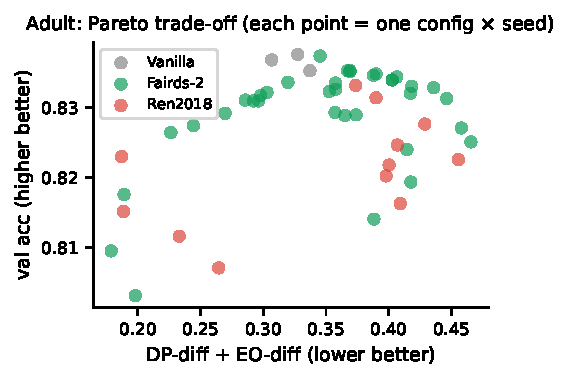
\includegraphics[width=0.55\textwidth]{figures/fig_pareto_adult.pdf}
  \caption{\textbf{Adult Pareto trade-off} (each point is one
  hyperparameter $\times$ seed). Vanilla and Ren2018($\eta\!=\!0.05$)
  jointly span the Pareto front; Fairds-2 is dominated.}
  \label{fig:pareto_adult}
\end{figure}

This is consistent with the Waterbirds result: in regimes where the
per-sample gradient is small or the benchmark itself does not benefit
from reweighting, closed-form Shapley reweighting cannot help.

\section{Spurious-strength phase transition}
\label{app:strength}

We sweep the spurious correlation strength $p_{\mathrm{maj}} \in
\{0.7, 0.8, 0.9, 0.95, 0.99\}$ on Colored MNIST, fixing all other
hyperparameters at the values used in §\ref{sec:exp:cmnist}, with 5
seeds. Figure~\ref{fig:strength_phase} shows that Fairds-2 is a
\emph{phase-dependent} winner: at weak spurious strengths
($p \leq 0.8$) all methods perform similarly, but as $p \to 0.99$
vanilla collapses (test\_worst $\to 0.19$) while Fairds-2 remains
robust at $0.74$. Paired one-sided $t$-tests:
$p_{\mathrm{maj}}\!=\!0.90$ \,$\Delta\!=\!+11.3$~pp ($p\!=\!0.011$);
$p_{\mathrm{maj}}\!=\!0.95$ \,$\Delta\!=\!+19.8$~pp ($p\!=\!0.021$);
$p_{\mathrm{maj}}\!=\!0.99$ \,$\Delta\!=\!+55.3$~pp ($p\!=\!3\!\times\!10^{-5}$).
This is the operating regime where the closed-form 2nd-order Shapley
reweighting most benefits worst-group robustness.

\begin{figure}[h]
  \centering
  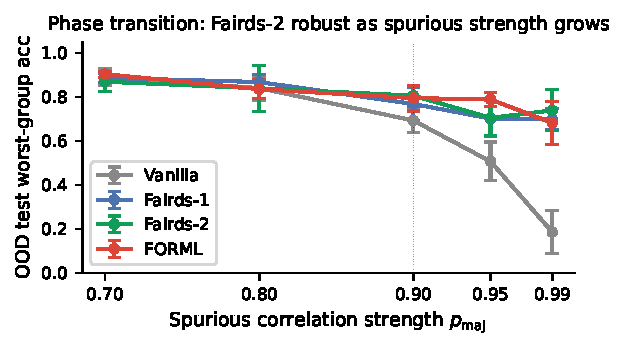
\includegraphics[width=0.6\textwidth]{figures/fig_strength_phase.pdf}
  \caption{\textbf{Phase transition with spurious strength.} Vanilla
  collapses at $p_{\mathrm{maj}} \geq 0.95$; Fairds-2 stays robust.}
  \label{fig:strength_phase}
\end{figure}

\section{RMS-rescaling ablation}
\label{app:rms_ablation}

Without the RMS rescaling described in Section~\ref{sec:method},
the 2nd-order Fairds variant collapses under strong spurious bias: on
the controlled spurious MLP at majority ratio $0.9$, $\alpha\!=\!0.5$
without rescaling drops accuracy to chance ($\sim\!0.50$). Once we
rescale the cross-term to match the per-batch RMS magnitude of the
first-order term, the same $\alpha$ produces the mechanism reported in
Section~\ref{sec:exp:e1b}. The 2nd-order term is otherwise dominated
by the magnitude of $H_{\mathrm{val}}$'s spectrum, which varies by
orders of magnitude over training.


\end{document}
